\documentclass[12pt,a4paper,english]{extarticle}
\usepackage[T1]{fontenc}
\usepackage[utf8]{inputenc}
\usepackage{fourier}
\usepackage{geometry}
\usepackage{multirow}
\geometry{verbose,tmargin=2.2cm,bmargin=2cm,lmargin=2.2cm,rmargin=2cm}
\usepackage{float}
\usepackage{textcomp}
\usepackage{amsmath}
\usepackage{stackrel}
\usepackage{graphicx}
\usepackage{esint}
\usepackage{tikz}
\usetikzlibrary{arrows, shapes.gates.logic.US, calc}
\tikzstyle{branch}=[fill, shape=circle, minimum size=3pt, inner sep=0pt]
\usetikzlibrary{matrix,calc}

\makeatletter

\providecommand{\tabularnewline}{\\}

\usepackage{fancyhdr}
\usepackage{lscape}
\usepackage{amssymb}
\pagestyle{fancy}
\lhead{Electronica III - 22.13}
\chead{TPL1}
\rhead{ITBA}
\renewcommand{\headrulewidth}{1pt}
\renewcommand{\footrulewidth}{1pt}

\makeatother

\usepackage[english]{babel}

\usepackage{tikz}
\usetikzlibrary{matrix,calc}

%isolated term
%#1 - Optional. Space between node and grouping line. Default=0
%#2 - node
%#3 - filling color
\newcommand{\implicantsol}[3][0]{
    \draw[rounded corners=3pt, fill=#3, opacity=0.3] ($(#2.north west)+(135:#1)$) rectangle ($(#2.south east)+(-45:#1)$);
    }


%internal group
%#1 - Optional. Space between node and grouping line. Default=0
%#2 - top left node
%#3 - bottom right node
%#4 - filling color
\newcommand{\implicant}[4][0]{
    \draw[rounded corners=3pt, fill=#4, opacity=0.3] ($(#2.north west)+(135:#1)$) rectangle ($(#3.south east)+(-45:#1)$);
    }

%group lateral borders
%#1 - Optional. Space between node and grouping line. Default=0
%#2 - top left node
%#3 - bottom right node
%#4 - filling color
\newcommand{\implicantcostats}[4][0]{
    \draw[rounded corners=3pt, fill=#4, opacity=0.3] ($(rf.east |- #2.north)+(90:#1)$)-| ($(#2.east)+(0:#1)$) |- ($(rf.east |- #3.south)+(-90:#1)$);
    \draw[rounded corners=3pt, fill=#4, opacity=0.3] ($(cf.west |- #2.north)+(90:#1)$) -| ($(#3.west)+(180:#1)$) |- ($(cf.west |- #3.south)+(-90:#1)$);
}

%group top-bottom borders
%#1 - Optional. Space between node and grouping line. Default=0
%#2 - top left node
%#3 - bottom right node
%#4 - filling color
\newcommand{\implicantdaltbaix}[4][0]{
    \draw[rounded corners=3pt, fill=#4, opacity=0.3] ($(cf.south -| #2.west)+(180:#1)$) |- ($(#2.south)+(-90:#1)$) -| ($(cf.south -| #3.east)+(0:#1)$);
    \draw[rounded corners=3pt, fill=#4, opacity=0.3] ($(rf.north -| #2.west)+(180:#1)$) |- ($(#3.north)+(90:#1)$) -| ($(rf.north -| #3.east)+(0:#1)$);
}

%group corners
%#1 - Optional. Space between node and grouping line. Default=0
%#2 - filling color
\newcommand{\implicantcantons}[2][0]{
    \draw[rounded corners=3pt, opacity=.3] ($(rf.east |- 0.south)+(-90:#1)$) -| ($(0.east |- cf.south)+(0:#1)$);
    \draw[rounded corners=3pt, opacity=.3] ($(rf.east |- 8.north)+(90:#1)$) -| ($(8.east |- rf.north)+(0:#1)$);
    \draw[rounded corners=3pt, opacity=.3] ($(cf.west |- 2.south)+(-90:#1)$) -| ($(2.west |- cf.south)+(180:#1)$);
    \draw[rounded corners=3pt, opacity=.3] ($(cf.west |- 10.north)+(90:#1)$) -| ($(10.west |- rf.north)+(180:#1)$);
    \fill[rounded corners=3pt, fill=#2, opacity=.3] ($(rf.east |- 0.south)+(-90:#1)$) -|  ($(0.east |- cf.south)+(0:#1)$) [sharp corners] ($(rf.east |- 0.south)+(-90:#1)$) |-  ($(0.east |- cf.south)+(0:#1)$) ;
    \fill[rounded corners=3pt, fill=#2, opacity=.3] ($(rf.east |- 8.north)+(90:#1)$) -| ($(8.east |- rf.north)+(0:#1)$) [sharp corners] ($(rf.east |- 8.north)+(90:#1)$) |- ($(8.east |- rf.north)+(0:#1)$) ;
    \fill[rounded corners=3pt, fill=#2, opacity=.3] ($(cf.west |- 2.south)+(-90:#1)$) -| ($(2.west |- cf.south)+(180:#1)$) [sharp corners]($(cf.west |- 2.south)+(-90:#1)$) |- ($(2.west |- cf.south)+(180:#1)$) ;
    \fill[rounded corners=3pt, fill=#2, opacity=.3] ($(cf.west |- 10.north)+(90:#1)$) -| ($(10.west |- rf.north)+(180:#1)$) [sharp corners] ($(cf.west |- 10.north)+(90:#1)$) |- ($(10.west |- rf.north)+(180:#1)$) ;
}

%Empty Karnaugh map 4x4
\newenvironment{Karnaugh}%
{
\begin{tikzpicture}[baseline=(current bounding box.north),scale=0.8]
\draw (0,0) grid (4,4);
\draw (0,4) -- node [pos=0.7,above right,anchor=south west] {ba} node [pos=0.7,below left,anchor=north east] {dc} ++(135:1);
%
\matrix (mapa) [matrix of nodes,
        column sep={0.8cm,between origins},
        row sep={0.8cm,between origins},
        every node/.style={minimum size=0.3mm},
        anchor=8.center,
        ampersand replacement=\&] at (0.5,0.5)
{
                       \& |(c00)| 00         \& |(c01)| 01         \& |(c11)| 11         \& |(c10)| 10         \& |(cf)| \phantom{00} \\
|(r00)| 00             \& |(0)|  \phantom{0} \& |(1)|  \phantom{0} \& |(3)|  \phantom{0} \& |(2)|  \phantom{0} \&                     \\
|(r01)| 01             \& |(4)|  \phantom{0} \& |(5)|  \phantom{0} \& |(7)|  \phantom{0} \& |(6)|  \phantom{0} \&                     \\
|(r11)| 11             \& |(12)| \phantom{0} \& |(13)| \phantom{0} \& |(15)| \phantom{0} \& |(14)| \phantom{0} \&                     \\
|(r10)| 10             \& |(8)|  \phantom{0} \& |(9)|  \phantom{0} \& |(11)| \phantom{0} \& |(10)| \phantom{0} \&                     \\
|(rf) | \phantom{00}   \&                    \&                    \&                    \&                    \&                     \\
};
}%
{
\end{tikzpicture}
}

%Empty Karnaugh map 2x4
\newenvironment{Karnaughvuit}%
{
\begin{tikzpicture}[baseline=(current bounding box.north),scale=0.8]
\draw (0,0) grid (4,2);
\draw (0,2) -- node [pos=0.7,above right,anchor=south west] {bc} node [pos=0.7,below left,anchor=north east] {a} ++(135:1);
%
\matrix (mapa) [matrix of nodes,
        column sep={0.8cm,between origins},
        row sep={0.8cm,between origins},
        every node/.style={minimum size=0.3mm},
        anchor=4.center,
        ampersand replacement=\&] at (0.5,0.5)
{
                      \& |(c00)| 00         \& |(c01)| 01         \& |(c11)| 11         \& |(c10)| 10         \& |(cf)| \phantom{00} \\
|(r00)| 0             \& |(0)|  \phantom{0} \& |(1)|  \phantom{0} \& |(3)|  \phantom{0} \& |(2)|  \phantom{0} \&                     \\
|(r01)| 1             \& |(4)|  \phantom{0} \& |(5)|  \phantom{0} \& |(7)|  \phantom{0} \& |(6)|  \phantom{0} \&                     \\
|(rf) | \phantom{00}  \&                    \&                    \&                    \&                    \&                     \\
};
}%
{
\end{tikzpicture}
}

%Empty Karnaugh map 2x2
\newenvironment{Karnaughquatre}%
{
\begin{tikzpicture}[baseline=(current bounding box.north),scale=0.8]
\draw (0,0) grid (2,2);
\draw (0,2) -- node [pos=0.7,above right,anchor=south west] {b} node [pos=0.7,below left,anchor=north east] {a} ++(135:1);
%
\matrix (mapa) [matrix of nodes,
        column sep={0.8cm,between origins},
        row sep={0.8cm,between origins},
        every node/.style={minimum size=0.3mm},
        anchor=2.center,
        ampersand replacement=\&] at (0.5,0.5)
{
          \& |(c00)| 0          \& |(c01)| 1  \\
|(r00)| 0 \& |(0)|  \phantom{0} \& |(1)|  \phantom{0} \\
|(r01)| 1 \& |(2)|  \phantom{0} \& |(3)|  \phantom{0} \\
};
}%
{
\end{tikzpicture}
}

%Defines 8 or 16 values (0,1,X)
\newcommand{\contingut}[1]{%
\foreach \x [count=\xi from 0]  in {#1}
     \path (\xi) node {\x};
}

%Places 1 in listed positions
\newcommand{\minterms}[1]{%
    \foreach \x in {#1}
        \path (\x) node {1};
}

%Places 0 in listed positions
\newcommand{\maxterms}[1]{%
    \foreach \x in {#1}
        \path (\x) node {0};
}

%Places X in listed positions
\newcommand{\indeterminats}[1]{%
    \foreach \x in {#1}
        \path (\x) node {X};
}

% \begin{document}
%     \begin{Karnaugh}
%         \contingut{0,0,0,0,0,0,0,0,0,0,0,0,0,0,0,0}
%        \implicant{0}{2}{red}
%        \implicant{5}{15}{purple}
%        \implicantdaltbaix[3pt]{3}{10}{blue}
%     \implicantcantons[2pt]{orange}
%        \implicantcostats{4}{14}{green}
%     \end{Karnaugh}
%     %
%     \begin{Karnaughvuit}
%        \minterms{3,4}
%         \maxterms{0,1,6,7}
%        \indeterminats{2,5}
%        \implicant{3}{2}{green}
%        \implicant{4}{5}{}
%     \end{Karnaughvuit}
%     %
%     \begin{Karnaughquatre}
%         \minterms{1,2}
%        \maxterms{0,3}
%        \implicantsol{1}{green}
%        \implicantsol{2}{red}
%     \end{Karnaughquatre}

% \end{document}

\usepackage{listings}
\newcommand{\horrule}[1]{\rule{\linewidth}{#1}}

\title{
        %\vspace{-1in} 	
        \usefont{OT1}{bch}{b}{n}
        \normalfont \normalsize \textsc{Instituto Tecnológico de Buenos Aires} \\ [25pt]
        \horrule{0.5pt} \\[0.4cm]
        \huge Trabajo Práctico de Laboratorio Nro. 2 \\
        \horrule{2pt} \\[0.5cm]
}
\author{
        \normalfont 								\normalsize
        NOWIK, Ariel 58309\\[-3pt]		\normalsize
        MASPERO, Martina 57120\\[-3pt]		\normalsize
        MESTANZA, Joaquin 58288\\[-3pt]		\normalsize
        REGUEIRA, Marcelo 58300\\[-3pt]		\normalsize
        \today
}
\date{}



%%% Begin document
\begin{document}
% The \input command appends the content of the file directly into the document.
\maketitle
\newpage


\section*{Task 3}

Given a truth table, it was requested to see what happens
when the truth table is implemented with the smallest quantity of logic
gates. To perform this task, ICs that have NAND logic gates only
 will be used. This is because in most of ICs there are many
logic gates so it's a waste of logic gates if we use for example
just one of them. Note that this can also be implemented with 
NOR only ICs.

\subsection*{Low cost approach}
\begin{figure}[htbp]
    \begin{center}
    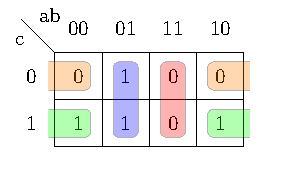
\includegraphics{data/karnaugh.pdf}
    
    \end{center}
    
    \caption{Karnaugh Map of the given truth table}
    \label{fig:KarnaughMap}
    \end{figure}
Let Z be the output label, its reduced minterms expression is:
\begin{equation}
    Z= (\bar{A}.B)+(C.\bar{B})
\end{equation} 
Also, its reduced maxterms expression is:
\begin{equation}
    Z= (\bar{A}+\bar{B}).(C+B)
\end{equation} 
\begin{figure}[htbp]
    \begin{center}
        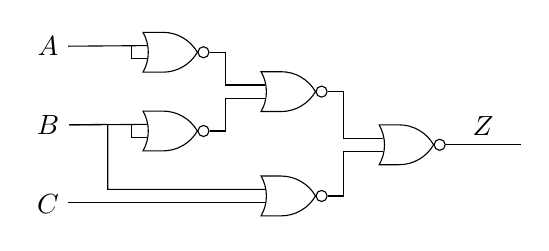
\begin{tikzpicture}
            %seteamos el orden de las variables
            \node (x) at (0, 2)(x) {$A$};
            \node (y) at (0, 1) (y){$B$};
            \node (z) at (0, 0)(z) {$C$};
        
            %creamos un nodo con una posicion asociada:($(x)) que es donde se encuentra
            %posicionada la variable x y le ponemos nombre: nor_x
            %los numeros son para desplazar la compuertas
            \node[nor gate US, draw, rotate=0, logic gate inputs=nn] at ($(x) + (1.5, -0.075)$) (nor_x) {};
            \node[nor gate US, draw, rotate=0, logic gate inputs=nn] at ($(y) + (1.5, -0.075)$) (nor_y) {};
            
            %dibujar la nor con las entradas unidas:
            %primero dibujamos una linea
            \draw (x) -- (nor_x.input 1); 
            % ahora dibujamos desplazada la linea que va a entrar al input 2
            \draw (nor_x.input 2) -- ([xshift=-0.2cm]nor_x.input 2) |- (nor_x.input 1);
        
            \draw (y) -- (nor_y.input 1);
            \draw (nor_y.input 2) -- ([xshift=-0.2cm]nor_y.input 2) |- (nor_y.input 1);
        
            %asigno dos entradas
            \node[nor gate US, draw, rotate=0, logic gate inputs=nn] at ($(x) + (3, -0.075-0.5)$) (norAndB) {};
            \draw (nor_x.output) -- ([xshift=0.2cm]nor_x.output) |- (norAndB.input 1);
            \draw (nor_y.output) -- ([xshift=0.2cm]nor_y.output) |- (norAndB.input 2);
        
            \node[nor gate US, draw, rotate=0, logic gate inputs=nn] at ($(z) + (3, 0+0.10)$) (norBandC) {};
            \draw (z) -- ([xshift=0.2cm]z) |- (norBandC.input 2);
            \draw (y) -- ([xshift=-0.5cm]nor_y.input 1)  |- (norBandC.input 1);
        
            \node[nor gate US, draw, rotate=0, logic gate inputs=nn] at ($(y) + (4.5, -0.25)$) (norFinal) {};
            \draw (norAndB.output) -- ([xshift=0.2cm]norAndB.output) |- (norFinal.input 1);
            \draw (norBandC.output) -- ([xshift=0.2cm]norBandC.output) |- (norFinal.input 2);
        
            \draw (norFinal.output) -- node[above]{$Z$} ($(norFinal) + (1.5, 0)$);
        \end{tikzpicture}
        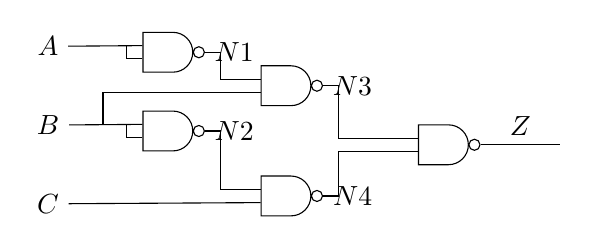
\begin{tikzpicture}
            \node (x) at (0, 2)(x) {$A$};
            \node (y) at (0, 1) (y){$B$};
            \node (z) at (0, 0)(z) {$C$};
            \node[nand gate US, draw, rotate=0, logic gate inputs=nn] at ($(x) + (1.5, -0.075)$) (nand_x) {};
            \draw (x) -- (nand_x.input 1); 
            \draw (nand_x.input 2) -- ([xshift=-0.2cm]nand_x.input 2) |- (nand_x.input 1);
            \draw (nand_x.output) -- node[right]{$N1$} ($(nand_x.output) + (0, 0)$);

            \node[nand gate US, draw, rotate=0, logic gate inputs=nn] at ($(x) + (3, -0.5)$) (nandAandB) {};
 


            \draw (nand_x.output) -- ([xshift=0.2cm]nand_x.output) |- (nandAandB.input 1) ;
            \node[nand gate US, draw, rotate=0, logic gate inputs=nn] at ($(y) + (1.5, -0.075)$) (nand_y) {};
            \draw (nand_y.output) -- node[right]{$N2$} ($(nand_y.output) + (0, 0)$);

            \draw (nandAandB.output) -- node[right]{$N3$} ($(nandAandB.output) + (0, 0)$);

            \draw (y) -- (nand_y.input 1); 
            \draw (nand_y.input 2) -- ([xshift=-0.2cm]nand_y.input 2) |- (nand_y.input 1);
            \draw (nand_y.input 1) -- ([yshift=0cm]nand_y.input 1) -- ([xshift=-0.5cm]nand_y.input 1) |- (nandAandB.input 2);
            \node[nand gate US, draw, rotate=0, logic gate inputs=nn] at ($(z) + (3,0.1)$) (nandBandC) {};
            
            \draw (nandBandC.output) -- node[right]{$N4$} ($(nandBandC) + (0.5, 0)$);
            
            \draw (z) -- (nandBandC.input 2); 
            \draw (nand_y.output) -- ([xshift=0.2cm]nand_y.output) |- (nandBandC.input 1);

            \node[nand gate US, draw, rotate=0, logic gate inputs=nn] at ($(y) + (5, -0.25)$) (nandFinal) {};
            \draw (nandAandB.output) -- ([xshift=0.2cm]nandAandB.output) |- (nandFinal.input 1);
            \draw (nandBandC.output) -- ([xshift=0.2cm]nandBandC.output) |- (nandFinal.input 2);
            \draw (nandFinal.output) -- node[above]{$Z$} ($(nandFinal) + (1.5, 0)$);

        \end{tikzpicture}



    \end{center}
    \caption{Implementation with NOR gates and NAND gates respectively}
\end{figure} 

Note that the quantity of logic gates in both cases are the same.

\section*{Hazards}

Sometimes propagation delays cause unexpected and unwanted transitions 
in the ouput. Depending on what we see in the output is how this issue is
called. If there is a transition from 1 to 0 and the output was supposed to
stay at 1 it is said that the circuit has a static 1-hazard. If the output must
go from 0 to 1(or 1 to 0) and before establishing at 1 (or 0), it changes its value 
it is said that the circuit has a dynamic hazard.

Hazards can always be found at the Karnaugh map.
An input that follows multiple paths to an output can create a glitch (due to the hazards in the circuit) if, for example, 
one path has an inverter (in this case implemented with a NAND logic gate) 
and one does not. This issue is called "asymmetric path delay" and it can be
seen in Figure~\ref{fig:KarnaughMap} with the input B. 

\begin{figure}[H] 
    \begin{center}
    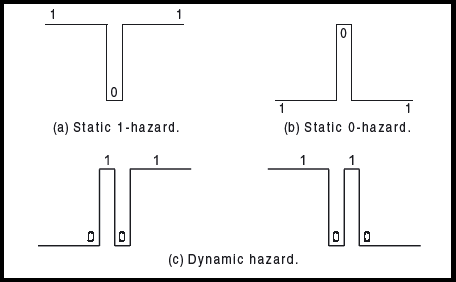
\includegraphics[width=0.45\textwidth]{data/hazard.png}
    \end{center}
    \caption{Different types of hazards}
    \label{fig:hazards}
    \end{figure} 



 \subsection*{Static 1-Hazard example} 
 Take the NAND implementation into account, assume all the propagation times 
 equal and then observe transition of the states A,B,C from 011 to 001 respectively.


\begin{figure}[H] 
    \begin{center}
    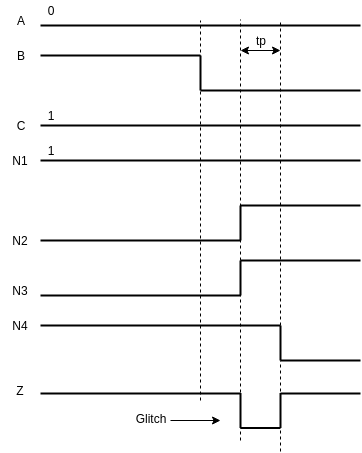
\includegraphics[width=6cm,height=8cm]{data/glitch.png}
    \end{center}
    \caption{Propagation time analysis}
    \label{fig:proptime}
    \end{figure} 
Note that tp in Figure~\ref{fig:proptime}  denotes the propagation time.

It can be seen that there should be a glitch at the output.The different combination of delays that produce a glitch may or may not be likely 
to occur in the implementation of the circuit. In some instances it is very 
unlikely that such delays would occur.


\section*{Measures obtained from NAND implementation}
\begin{figure}[H] 
\begin{center}
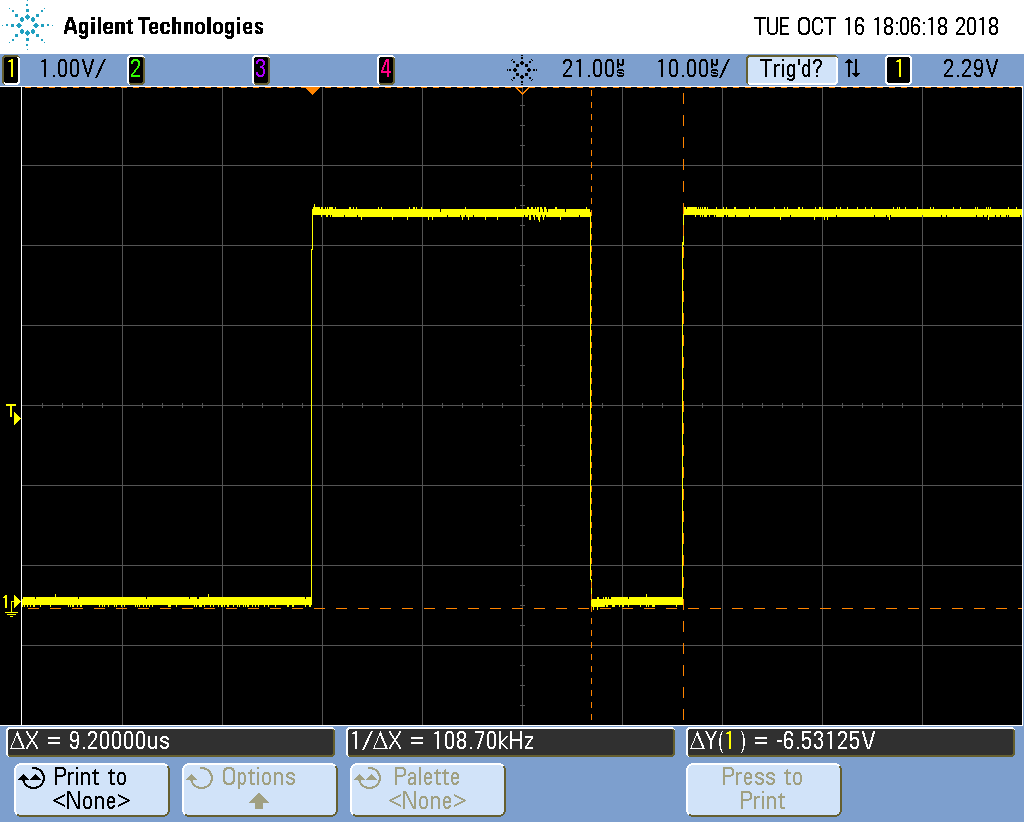
\includegraphics[width=8.25cm,height=8cm]{data/000to001.png}
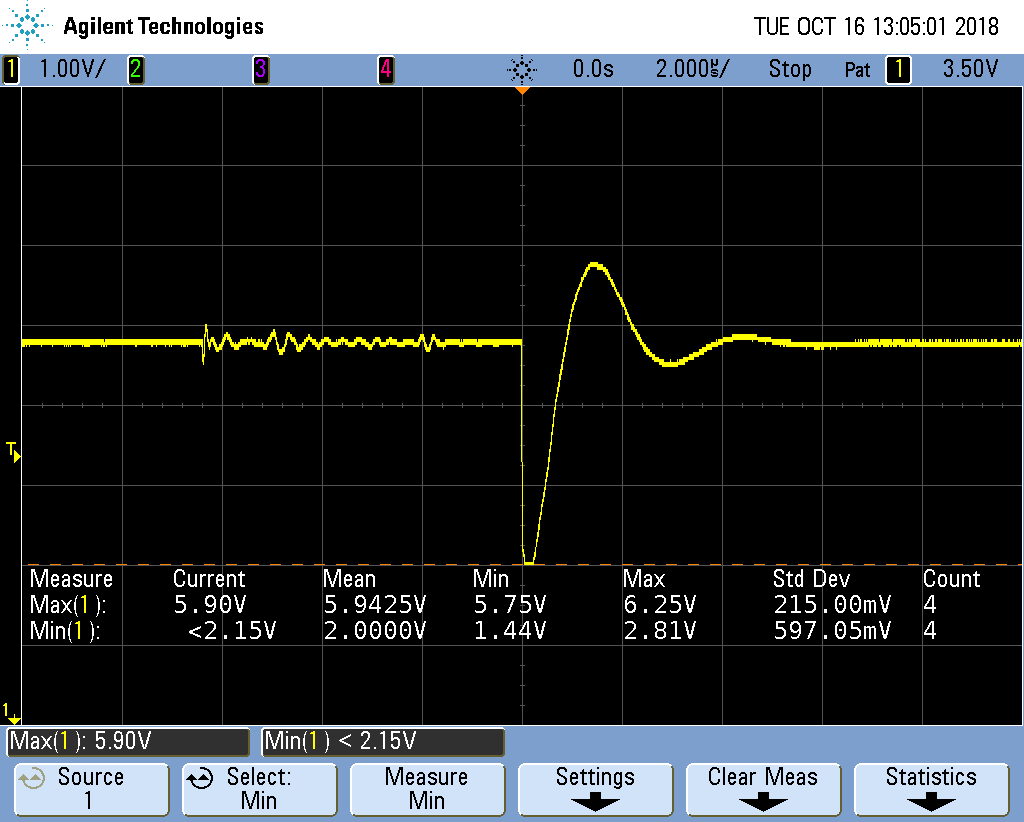
\includegraphics[width=8.25cm,height=8cm]{data/001to011.png}
\end{center}
\caption{Dynamic hazard and static 1-hazard respectively}
\label{fig:measures}
\end{figure} 

\section*{Conclusion}
In order to remove glitches it is needed to add redundant groups in the
Karnaugh Map so that disjoint groups overlap.
\begin{figure}[H] 
    \begin{center}
    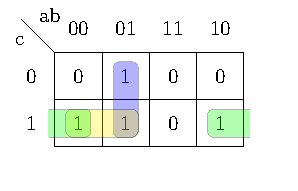
\includegraphics{data/karnaugh_improved.pdf}
    \end{center}
    \caption{Karnaugh with redundant logic}
    \label{fig:karnaugh_improved}
    \end{figure} 
In this case the output is given by:
\begin{equation*}
    Z= (\bar{A}+\bar{B}).(C+B)+(\bar{A}.C)    
\end{equation*} 

Note that the new term term of the expression is not dependent
of B so regardless of the variation of B there won't be glitches
in the output.


%Task 4
\newpage

\section*{Task 4}
In this section, there are measured the 
propagation delay, rise time and fall time of
 a 74HC02 logic gate (CMOS tecnology) in 
 several configurations: without load, and with
  a circuit load as shown below.
  
  \begin{figure}[H]
    \begin{centering}
    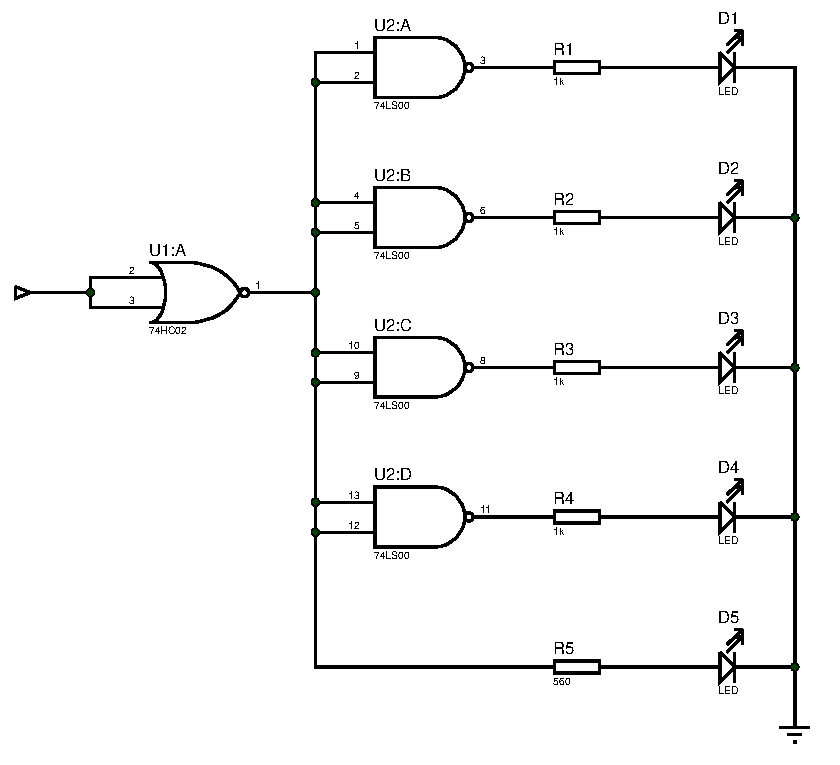
\includegraphics[width=0.7\textwidth]{data/circuitLED}
    \par\end{centering}
    \caption{Circuit load schematic - Made in Proteus 7.8}
\end{figure}

In the following table are the measured times
for the diferent configurations.

\begin{table}[H]
    \begin{center}
    \begin{tabular}{|c|c|c|c|c|}
    \hline
    CASE & $tpd_{L-H}$ & $tpd_{H-L}$ & $t_r$ & $t_f$\\
    \hline \hline
    Without LOAD & & & &  \\ \hline
    Circuit LOAD & & & & \\ \hline
    Circuit LOAD (100KHz) & & & & \\ \hline
    Circuit LOAD (100KHz with Capacitors) & & & & \\ \hline
    \end{tabular}
    \caption{Measured times}
    \end{center}
\end{table}

CONCLUSIONES DE TEMPERATURA, TIEMPOS Y EL PORQUE
DE USAR 100nF.




\newpage

\section*{Task 6}
In this section, a D Flip-Flop and a SR Latch
are implemented, based on logic gates.
\subsection*{SR Latch}
For the SR Latch, it is 
implemented using NOR gates of 74HC02 integrated
circuit. The resulting schematic is shown below.

\begin{figure}[H]
    \begin{centering}
    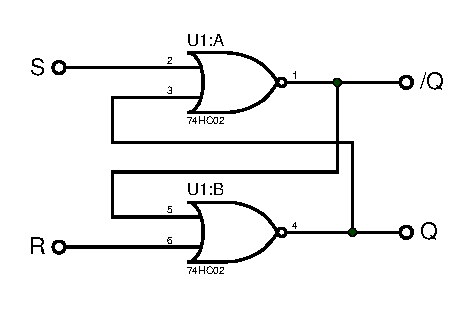
\includegraphics[width=0.5\textwidth]{data/latchSR}
    \par\end{centering}
    \caption{SR Latch circuit - Made in Proteus 7.8}
\end{figure}

The measured parameters are the same indicated
by the reference IC 74HC279\footnote{"TC74HC279AP", Toshiba, 1997-08-07} (Quad-SR-Latch): 
time propagation delays $(t_{pd})$ from S to Q, 
and from R to Q, for comparative purposes.

\begin{table}[H]
    \begin{center}
        \begin{tabular}{|c|c|c|c|c|}
            \hline 
            \multicolumn{2}{|c|}{PARAMETER} & FROM & TO & VALUE\tabularnewline
            \hline 
            \hline 
            \multirow{2}{*}{$t_{pd}$} & Circuit & S & Q & 13.2ns \tabularnewline
            \cline{2-5} 
             & 74HC279 & S & Q & 9ns\tabularnewline
            \hline 
            \multirow{2}{*}{$t_{pd}$} & Circuit & R & Q & 18ns \tabularnewline
            \cline{2-5} 
             & 74HC279 & R & Q & 11ns\tabularnewline
            \hline 
            \end{tabular}
    \caption{Measured values}
    \end{center}
\end{table}
As shown, the IC times are faster than the 
discrete latch builded. This diferences are 
related to the fact that the logic gates are 
not identical to each other, son they may have
diferent propagation delay times.\\
On the other side, with the Quad-NOT gate IC 74HC02 
only two latches can be built, in comparison with 
the four latches included in the 74HC279 IC.
\newpage
\subsection*{D Flip-Flop}
For the D flip-flop, it is implemented using 
the SR Latch designed before, adding the 
remaining parts as shown below.

\begin{figure}[H]
    \begin{centering}
    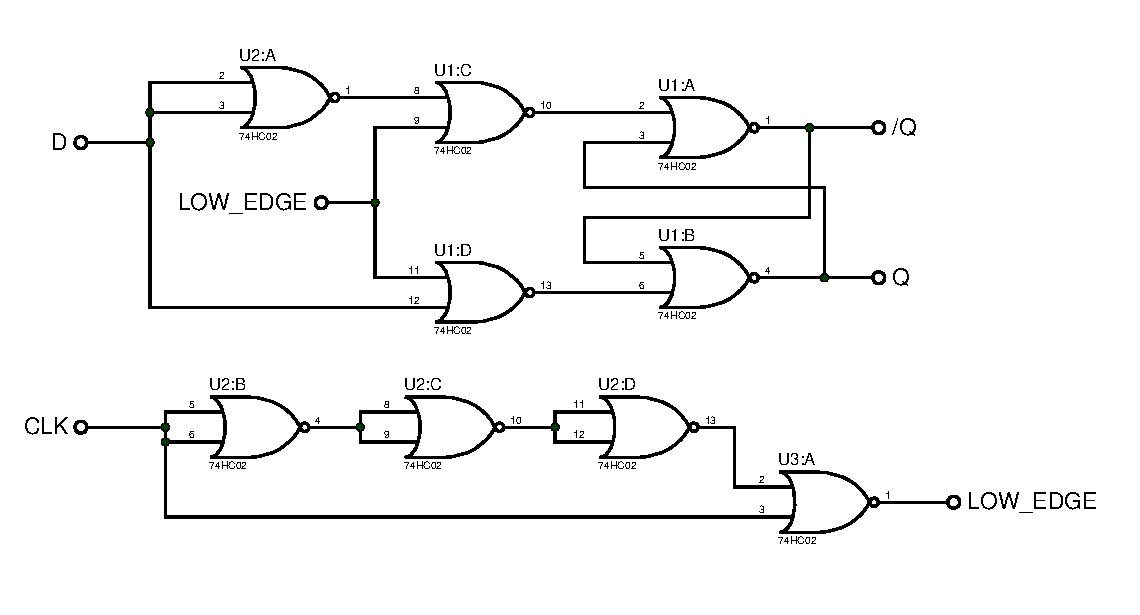
\includegraphics[width=0.8\textwidth]{data/dflipflop}
    \par\end{centering}
    \caption{D Flip-Flop circuit - Made in Proteus 7.8}
\end{figure}

The designed circuit will be compared with the 
74HC74\footnote{"74HC74 Dual D-type flip-flop with set and reset; positive edge-trigger", Nexperia, Rev.5 - 3 December 2015} D Flip-Flop.

\begin{table}[H]
    \begin{center}
        \begin{tabular}{|c|c|c|c|c|}
            \hline 
            \multicolumn{2}{|c|}{PARAMETER} & FROM & TO & VALUE\tabularnewline
            \hline 
            \hline 
            \multirow{2}{*}{$t_{pd}$} & Circuit & CLK & Q or /Q & 30ns\tabularnewline
            \cline{2-5} 
             & 74HC74 & CLK & Q or /Q & 14ns\tabularnewline
            \hline 
            \multirow{2}{*}{$t_t$} & Circuit &  & Q or /Q & 18ns \tabularnewline
            \cline{2-5} 
             & 74HC74 &  & Q or /Q & 7ns\tabularnewline
            \hline 
            \end{tabular}
    \caption{Measured values}
    \end{center}
\end{table}
As shown, the measured times from the built circuit 
are slower than the IC 74HC74 times. Also, it 
required two NOR-Gates IC (74HC02) to build the 
flip flop with all discrete logic gates, and 
each gate has its own time propagation delay that
needs to be considerated. On the other hand, the 
74HC74 has two flip flops in one IC; to build them 
with logic gates, 4 IC 74HC02 would be needed.

%Task 8
\newpage

\section*{Task 8}
In this section, a distance measurement system is 
implemented using discrete logic and the ultrasonic 
sensor HC - SR04. With it, distances between 1.7cm 
and 4.25m can be measured. The design is shown in 
the following block diagram.

\begin{figure}[H]
    \begin{centering}
    
\includegraphics[width=1\textwidth]{data/blockDiagram}
    \par\end{centering}
    \caption{Distance measurement system - Block diagram}
\end{figure}

\subsection*{Trigger Enable Logic}
For this part, a T flip-flop is used to
define two states: $(1)$ Measure enabled and $(2)$ Measuring.
\par
In state $(1)$, with TRIGGER\_EN on HIGH level, a measure 
can be made by sending a positive edge to the TRIGGER input, 
then the flip-flop changes to state $(2)$, preventing a new 
retrigger while measuring if a new positive edge is detected 
in TRIGGER input. This two states and the MEASURE\_READY bit 
are referenced from the $\overline{Q}$ output of the flip-flop. 
When the measure ends, an edge is sended to 
the CLR pin of the flip-flop, for returning to state $(1)$, allowing
to make a new measure. The previus performance is shown in the 
following time diagram.

\begin{figure}[H]
    \begin{centering}
    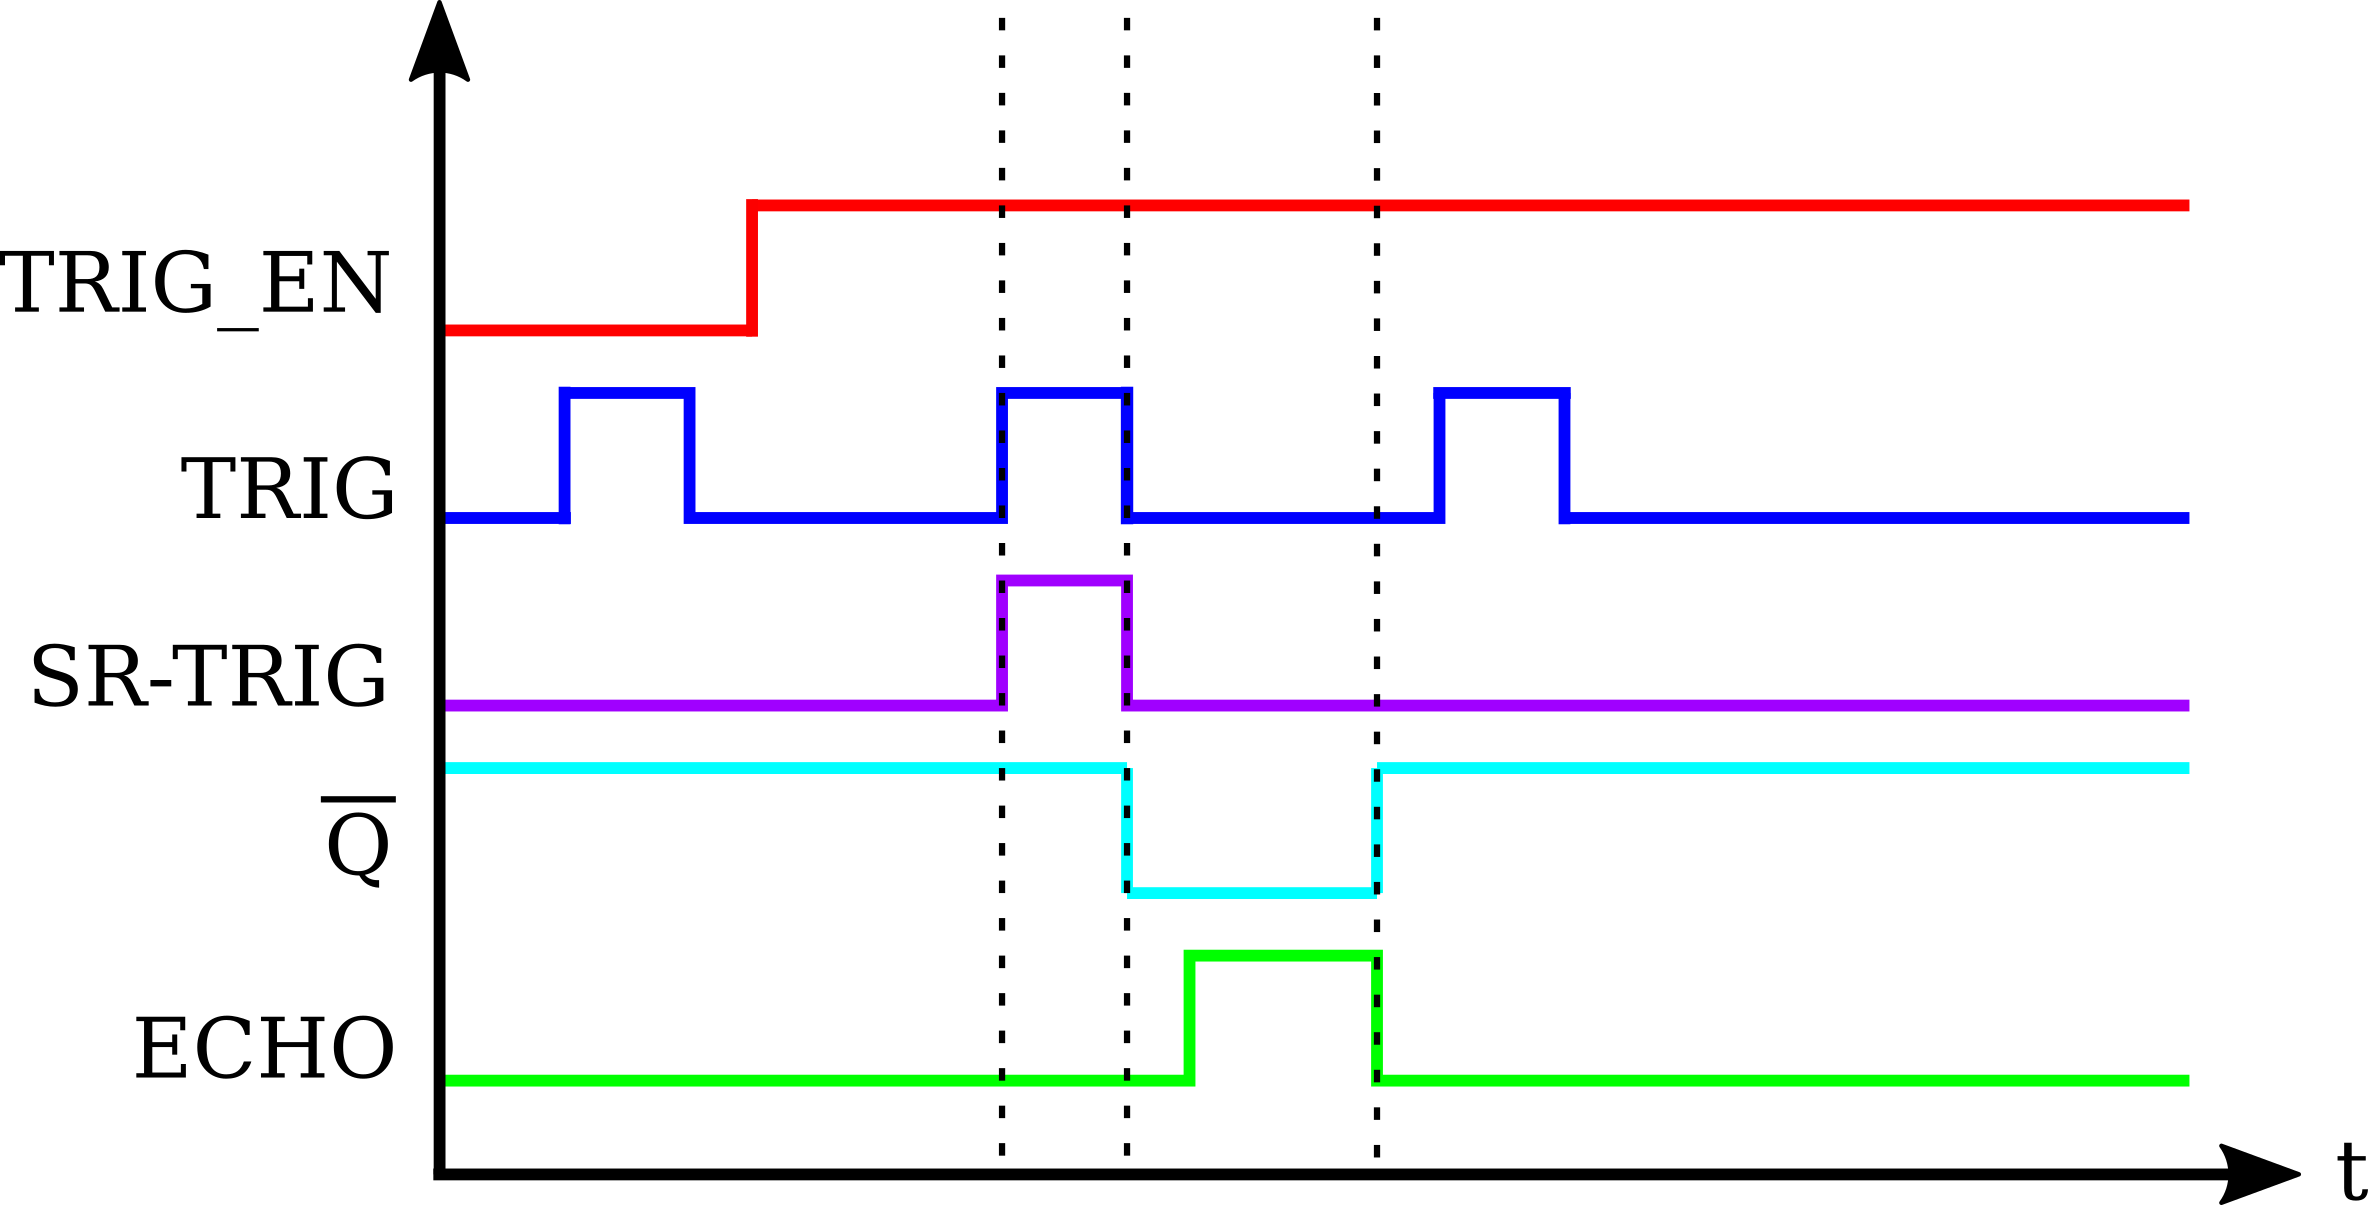
\includegraphics[width=0.7\textwidth]{data/trigerEnable_Time}
    \par\end{centering}
    \caption{Trigger Enable Logic - Time diagram}
\end{figure}
\newpage
The ultrasonic sensor needs a pulse of a period T > 10$\mu$Seg, 
so the edge of TRIGGER input is sended to a monostable circuit
(implemented with a LM555 timer) to ensure that the condition is met.
The final schematic of this section is shown below.

\begin{figure}[H]
    \begin{centering}
        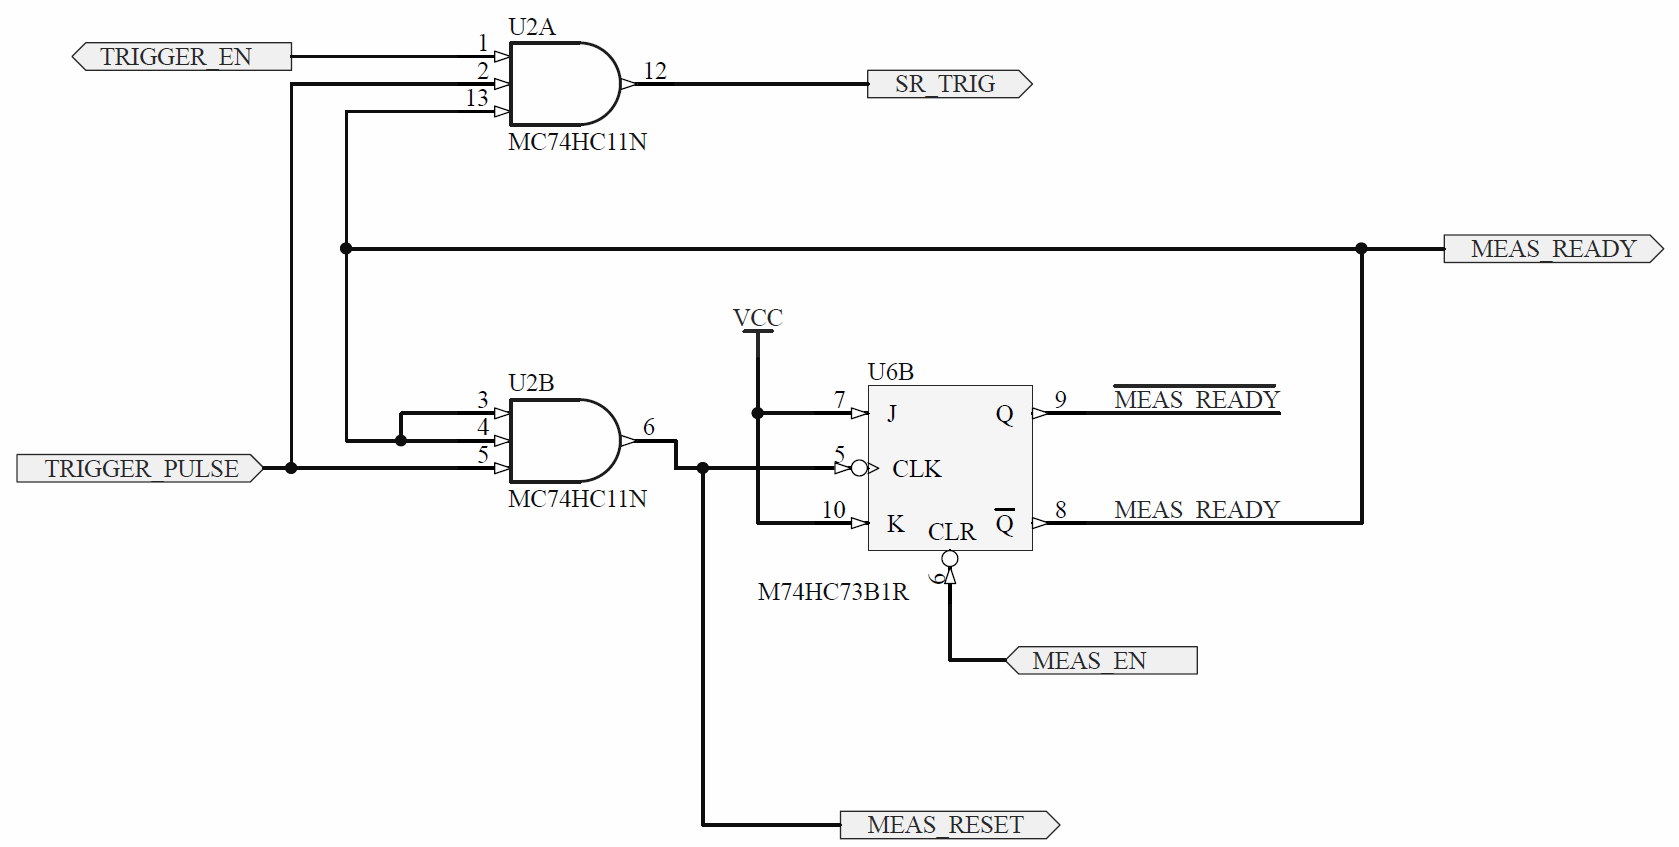
\includegraphics[width=1\textwidth]{data/trig_enable}
    \par\end{centering}
    \caption{Trigger Enable Logic - Schematic circuit made in Altium 15}
\end{figure}

\subsection*{HC - SR04 Sensor}
To make the measures in the mentioned interval, the HC - SR04 
after receiving the TRIG input pulse, it answers at the ECHO out 
with a pulse of a period T > 100$\mu$Seg (1.7cm), up to 25000$\mu$Seg (4.25m).
It will be fractioned in units of 100$\mu$Seg (to be counted).
\par
To know the measure value, the obtained number $N$ is processed in the
following calculation:
\[
    Distance[m] = 170 \cdot 100 \cdot 10^{-6} \cdot N  
\]
By fractioning the ECHO pulse in discrete units, the resulting resolution is
equivalent to 1.7cm, which is the smallest unit that can be counted (100$\mu$Seg).

\subsection*{Measure units detector}

For fractioning the ECHO response into units of 100$\mu$Seg, it is 
connected to an AND gate with a clock source (CLK) whose period is 100$\mu$Seg.\\
In this way, while the ECHO out stays at HIGH level, the signal at the AND gate output 
is equal to the clock source. While not measuring, the output stays at LOW level.
The previous performance is shown in the time diagram below.

\begin{figure}[H]
    \begin{centering}
    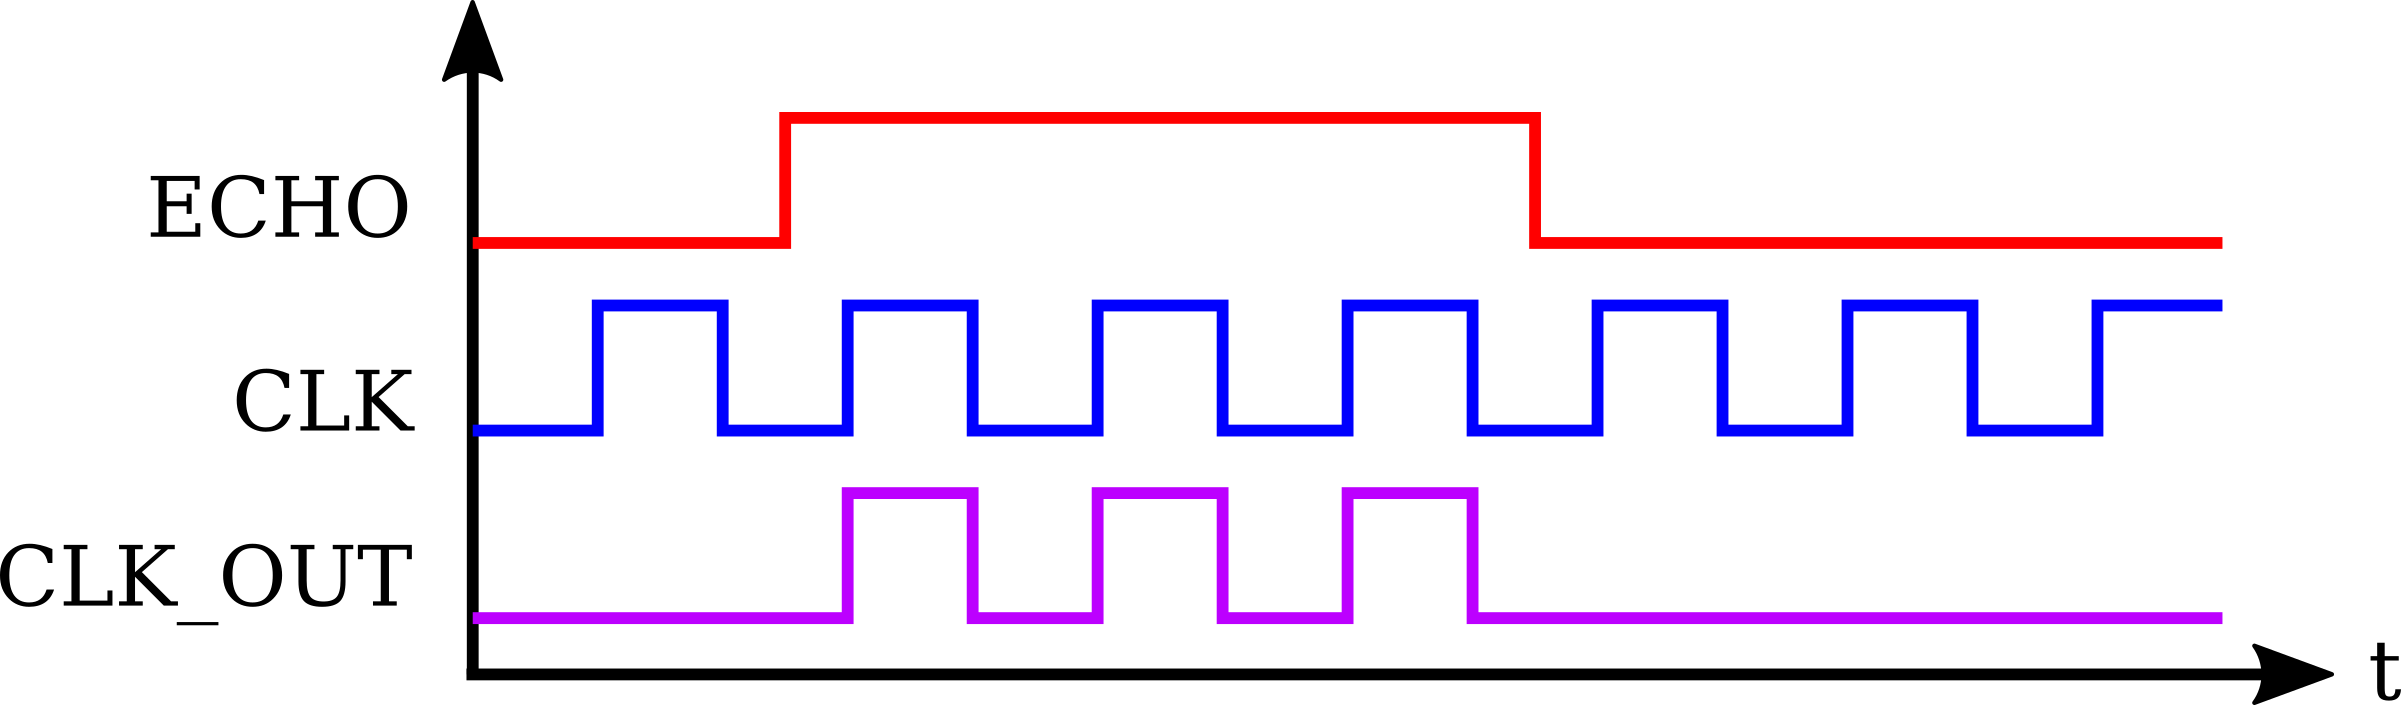
\includegraphics[width=0.65\textwidth]{data/CLK_time}
    \par\end{centering}
    \caption{Measure units detector - Time diagram}
\end{figure}

The CLK signal was implemented with a LM555 timer in astable configuration.
The schematic for this section is shown below.

\begin{figure}[H]
    \begin{centering}
    
\includegraphics[width=0.6\textwidth]{data/Unit_Detector}
    \par\end{centering}
    \caption{Measure units detector - Schematic circuit made in Altium 15}
\end{figure}

\subsection*{Synchronous counter}

For counting the time units, an integrated synchronous counter is implemented (CD4040), 
whose CLK input is conected to the out signal of the measure units detector. It detects the 
positive edges of the CLK signal, in this case having one per 100$\mu$Seg. From the 12-bit 
output, only 8-bit are used, because for measuring the maximum distance, only 250 untis are 
needed (25000$\mu$Seg over 100$\mu$Seg results in 250 units), and if the binary out is converted 
to decimal, the maximun number is $2^8 = 256$ (which covers the 250 maximum).\\
The integrated circuit implementation is shown below.

\begin{figure}[H]
    \begin{centering}
    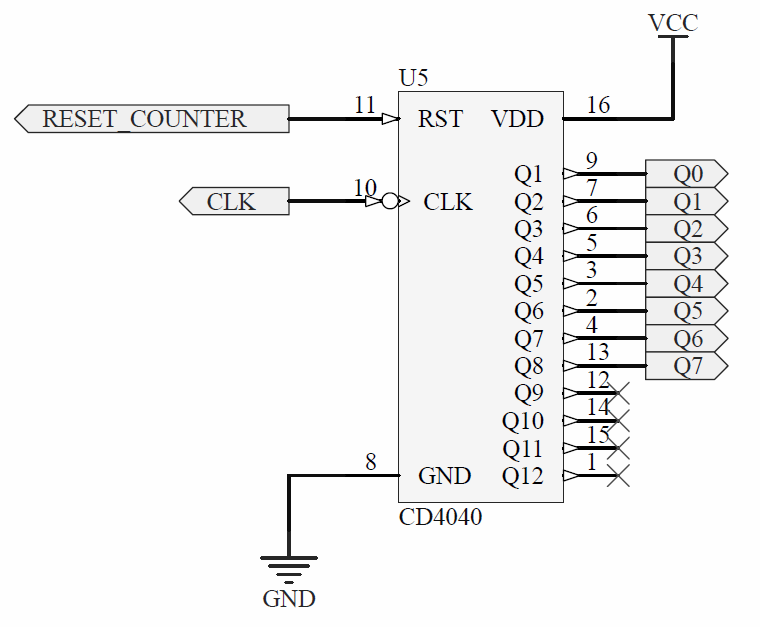
\includegraphics[width=0.5\textwidth]{data/Unit_Counter}
    \par\end{centering}
    \caption{Synchronous counter - Schematic circuit made in Altium 15}
\end{figure}

\subsection*{End of measure detector}

When the measure ends, the negative edge produced by the ECHO is used in a discrete edge detector 
to reset the flip-flop in the trigger enable logic, so a new measure can be started at any time.
The circuit diagram of the implementation is shown below.

\begin{figure}[H]
    \begin{centering}
    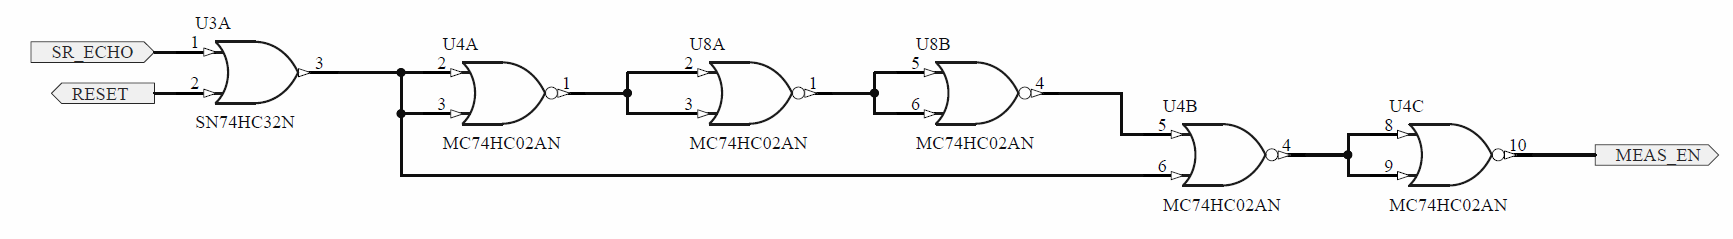
\includegraphics[width=1\textwidth]{data/Meas_End}
    \par\end{centering}
    \caption{End of measure detector - Schematic circuit made in Altium 15}
\end{figure}

The binary output resulting from the measure stays on until a new positive edge from the trigger is 
received. Then, the pulse used to change the flip-flop state in a new measure is also used to reset
the previous binary output from the synchronous counter.

\subsection*{Manual reset}

If when connecting the power supply to the circuit, the counter is not in cero, or the flip-flop starts 
switched into the state $(2)$, a manual switch for reset is added with a pull-down resistor, as shown below.

\begin{figure}[H]
    \begin{centering}
    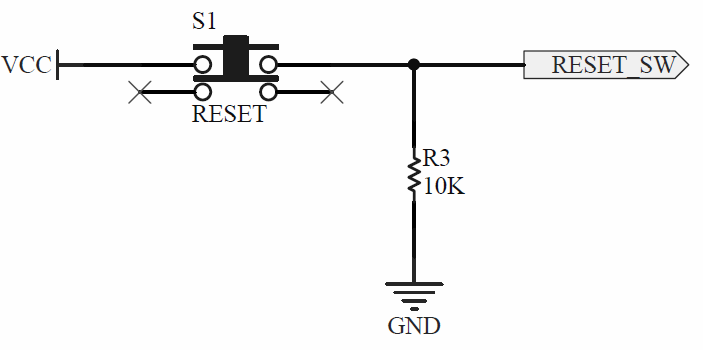
\includegraphics[width=0.5\textwidth]{data/pullDown_Switch}
    \par\end{centering}
    \caption{Manual reset with pull-down resistor - Made in Altium 15}
\end{figure}

\subsection*{Aditional settings}
\subsubsection*{MEASURE\_READY indicator}

To know if the flip-flop starts in the correct state when connecting the power supply or 
if the last measure has finished, 
a bicolor LED was used through two transistors, using the $Q$ and $\overline{Q}$ outputs 
of the flip-flop. When a measure ends (or when at the power supply connection the flip-flop starts
at the correct state), the LED turns green as an OK indication. When measuring, the LED turns red until
it ends. If when connecting the power supply (or in any moment) the flip-flop starts in the 
wrong state, the LED will remain in red. This can be fixed by pressing the reset switch.\\
The schematic circuit is shown below.

\begin{figure}[H]
    \begin{centering}
    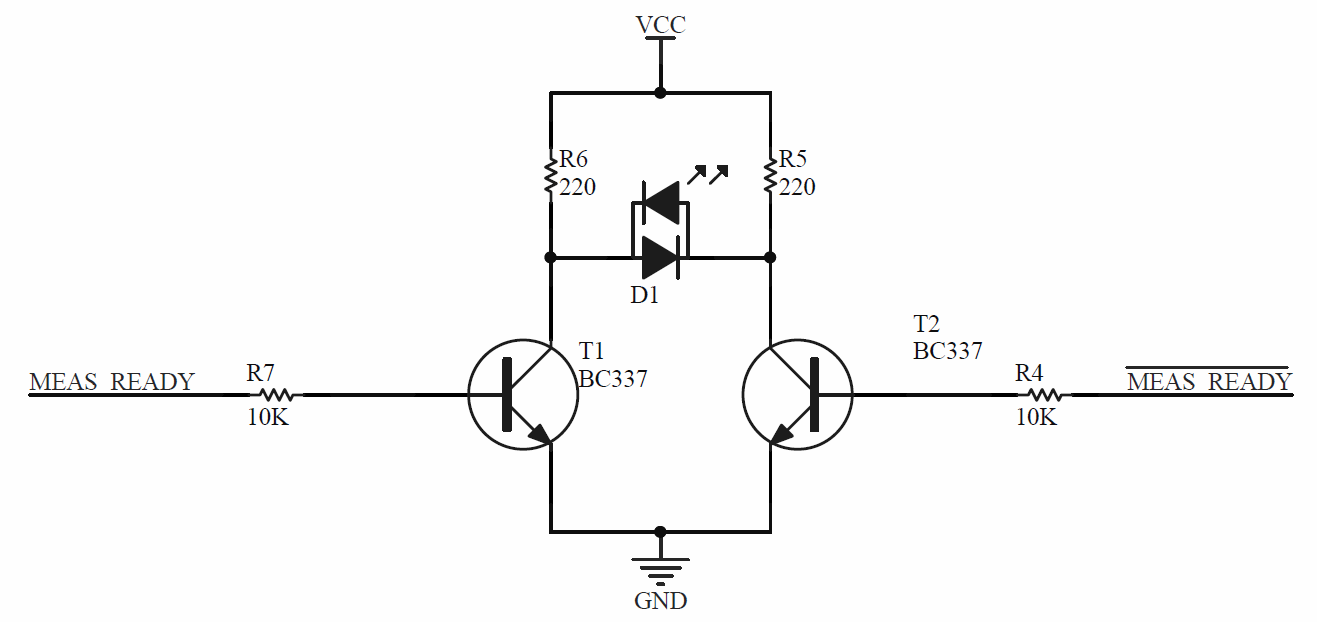
\includegraphics[width=0.9\textwidth]{data/Transistor_LogicLED}
    \par\end{centering}
    \caption{MEASURE\_END indicator - Transistor logic made in Altium 15}
\end{figure}
The calculation of the resistors can be read from the Annex.

\subsubsection*{Measure counted units indicator}

To obtain the amount of time units measured more easily, the CLK out of the
measure units detector is used in decade counters implemented with CD4033, because 
their out pins are decoded for use in 7-segment displays. Since the maximum measure 
has 3 digits, there are 3 counters and displays implemented (their reset pin is 
connected to the reset signal of the end of measure detector, and to the reset switch 
through an OR gate). The implemented circuit schematic is shown below. It has been done in 
a separete PCB.

\begin{figure}[H]
    \begin{centering}
    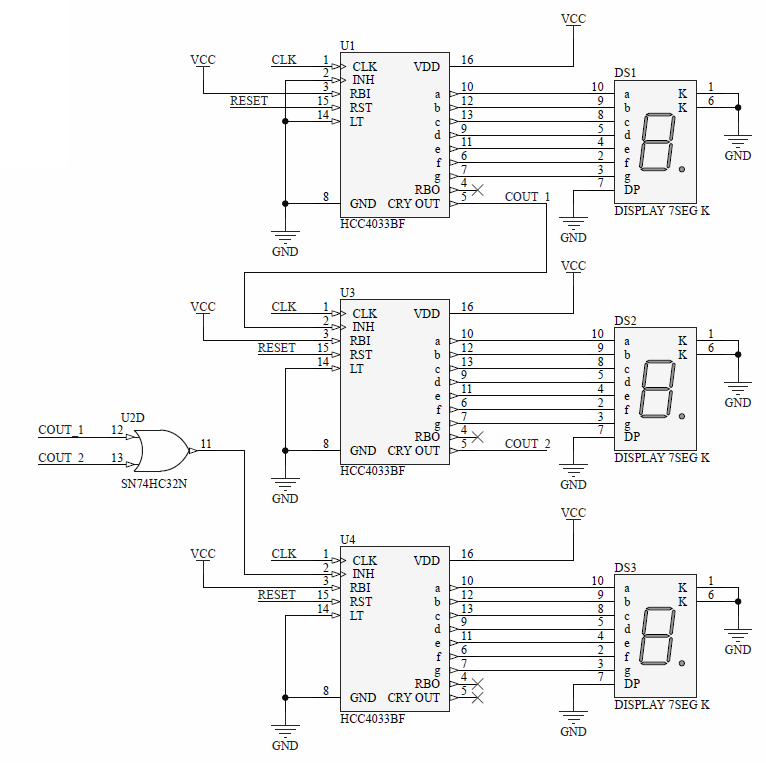
\includegraphics[width=1\textwidth]{data/Display}
    \par\end{centering}
    \caption{Measure display - Schematic circuit made in Altium 15}
\end{figure}

\newpage 
\section*{Appendix}
\subsection*{MEASURE\_READY indicator - Resistors calculation}

For the circuit design, the transistors are used in saturation-cutt off mode. 
Considering a $15mA$ current for the LED, it will be the $IC_{SAT}$. Going through 
the out loop we have:
\[
    V_{CC} - IC_{SAT}R_C - V_{LED} - VCE_{SAT} = 0    
\]
Considering as $VCE_{SAT} = 0.2V$ and a $V_{LED} = 1.8V$, the value of $R_C$ (collector resistor) can be obtained as follows:
\[
    \frac{V_{CC} - V_{LED} - VCE_{SAT}}{IC_{SAT}} = RC = 200 \Omega    
\]
Normalizing the value, it remains as $R_C = 220\Omega $. Recalculating the new $IC_{SAT}$:
\[
    \frac{V_{CC} - V_{LED} - VCE_{SAT}}{R_C} = IC_{SAT} = 13.6mA   
\]
Using the BC337 transistors, according to ON Semiconductor datasheet, the minimum HFE is 100, which will 
be used to calculate the minimum $IB_{SAT}$ (because its the worst case, to guarantee the saturation):
\[
    \frac{IC_{SAT}}{HFE_{MIN}} = IB_{SAT-MIN} = 136\mu A    
\]
With that value, the base resistors can be calculated, and then normalized down to get an $IB_{SAT}$ over 
the previous limit. Going through the entry loop:
\[
    V_{Q-OUT} - VBE_{ON} - IB_{SAT}R_B = 0
\]
Considerating that $VBE_{ON} = 0.7V$ and the output voltage of the flip-flop as $5V$ on HIGH level:
\[
    \frac{V_{Q-OUT} - VBE_{ON}}{IB_{SAT}} = RB_{MAX} = 31.6K\Omega    
\]
Normalizing the value, it results in $R_B = 10 K \Omega$. Checking the resulting $IB_{SAT}$:
\[
    \frac{V_{Q-OUT} - VBE_{ON}}{R_B} = IB_{SAT} = 436\mu A   
\]
According to maximun ratings of Texas Instruments datasheet, the $Q$ and $\overline{Q}$ outs can manage a current
up to $25mA$, so the resulting $IB_{SAT}$ is in range.





%%% End document
\end{document}
